\section{Appendix: Massively Multitask Networks for Drug Discovery}

\subsection{Dataset Construction and Design}

The PCBA datasets are dose-response assays performed by the NCATS Chemical Genomics Center (NCGC) and downloaded from PubChem BioAssay using the following search limits: TotalSidCount from 10000, ActiveSidCount from 30, Chemical, Confirmatory, Dose-Response, Target: Single, NCGC. These limits correspond to the search query: (10000[TotalSidCount] :
1000000000[TotalSidCount]) AND (30[ActiveSidCount] :
1000000000[ActiveSidCount]) AND ``small\_molecule''[filt] AND
``doseresponse''[filt] AND 1[TargetCount] AND ``NCGC''[SourceName].  We note that the DUD-E datasets are especially susceptible to ``artificial enrichment'' (unrealistic divisions between active and inactive compounds) as an artifact of the dataset construction procedure. Each data point in
our collection was associated with a binary label classifying it as either active or inactive.

A description of each of our 259 datasets is given in \tablename~A1.  These datasets cover a wide range of target classes and assay types, including both cell-based and in vitro experiments. Datasets with duplicated targets are marked with an asterisk (note that only the non-DUD-E duplicate target datasets were used in the analysis described in the text). For the PCBA datasets, compounds not labeled ``Active'' were considered inactive (including compounds marked ``Inconclusive''). Due to missing data in PubChem BioAssay and/or featurization errors, some data points and compounds were not used for evaluation of our models; failure rates for each dataset group are shown in \tablename~\ref{tab:failures}. The Tox21 group suffered especially high failure rates, likely due to the relatively large number of metallic or otherwise abnormal compounds that are not supported by the RDKit package.  The counts given in \tablename~A1 do not include these missing data. A graphical breakdown of the datasets by target class is shown in \figurename~\ref{fig:target_bar}. The datasets used for the held-in and held-out analyses are repeated in \tablename~\ref{tab:held-in} and \tablename~\ref{tab:held-out}, respectively.

As an extension of our treatment of task similarity in the text, we generated the heatmap in \figurename~\ref{fig:dataset_heatmap} to show the pairwise intersection between all datasets in our collection. A few characteristics of our datasets are immediately apparent: \begin{itemize} 
\item The datasets in the DUD-E group have very little intersection with any other datasets.
\item The PCBA and Tox21 datasets have substantial
self-overlap. In contrast, the MUV datasets have relatively little
self-overlap.  \item The MUV datasets have substantial overlap with the
datasets in the PCBA group.  \item The Tox21 datasets have very small
intersections with datasets in other groups.  \end{itemize}

\figurename~\ref{fig:duplicates} shows the $\Delta$ log-odds-mean-AUC for
datasets with duplicate and unique targets.

\afterpage{%
\clearpage% Flush earlier floats (otherwise order might not be correct)
\thispagestyle{empty}% empty page style (?)
\begin{landscape}% Landscape page
\centering % Center table
\rowcolors{2}{gray!25}{white}
\csvreader[
longtable=lSSlp{1.3in},
table head={\toprule\bfseries Dataset & \bfseries Actives & \bfseries Inactives & \bfseries Target Class & \bfseries Target \\
\midrule\endhead\bottomrule\endfoot},
]
{Data/datasets.csv}{1=\Dataset, 2=\Actives, 3=\Inactives, 4=\Class, 5=\Target}{\Dataset & \Actives & \Inactives & \Class & \Target}

\begin{table}[ht]
\centering
\caption{Featurization failures.}
\label{tab:failures}
\vskip 0.2in
\begin{tabular}{|c|c|c|c|}
\toprule
Group & \text{Original} & \text{Featurized} & \text{Failure Rate (\%)} \\
\midrule
PCBA & 439879 & 437928 & 0.44 \\
DUD-E & 1200966 & 1200406 & 0.05 \\
MUV & 95916 & 95899 & 0.02 \\
Tox21 & 11764 & 7830 & 33.44 \\
\bottomrule
\end{tabular}
\end{table}
\end{landscape}
\clearpage% Flush page
}

\begin{figure}[ht]
\centering
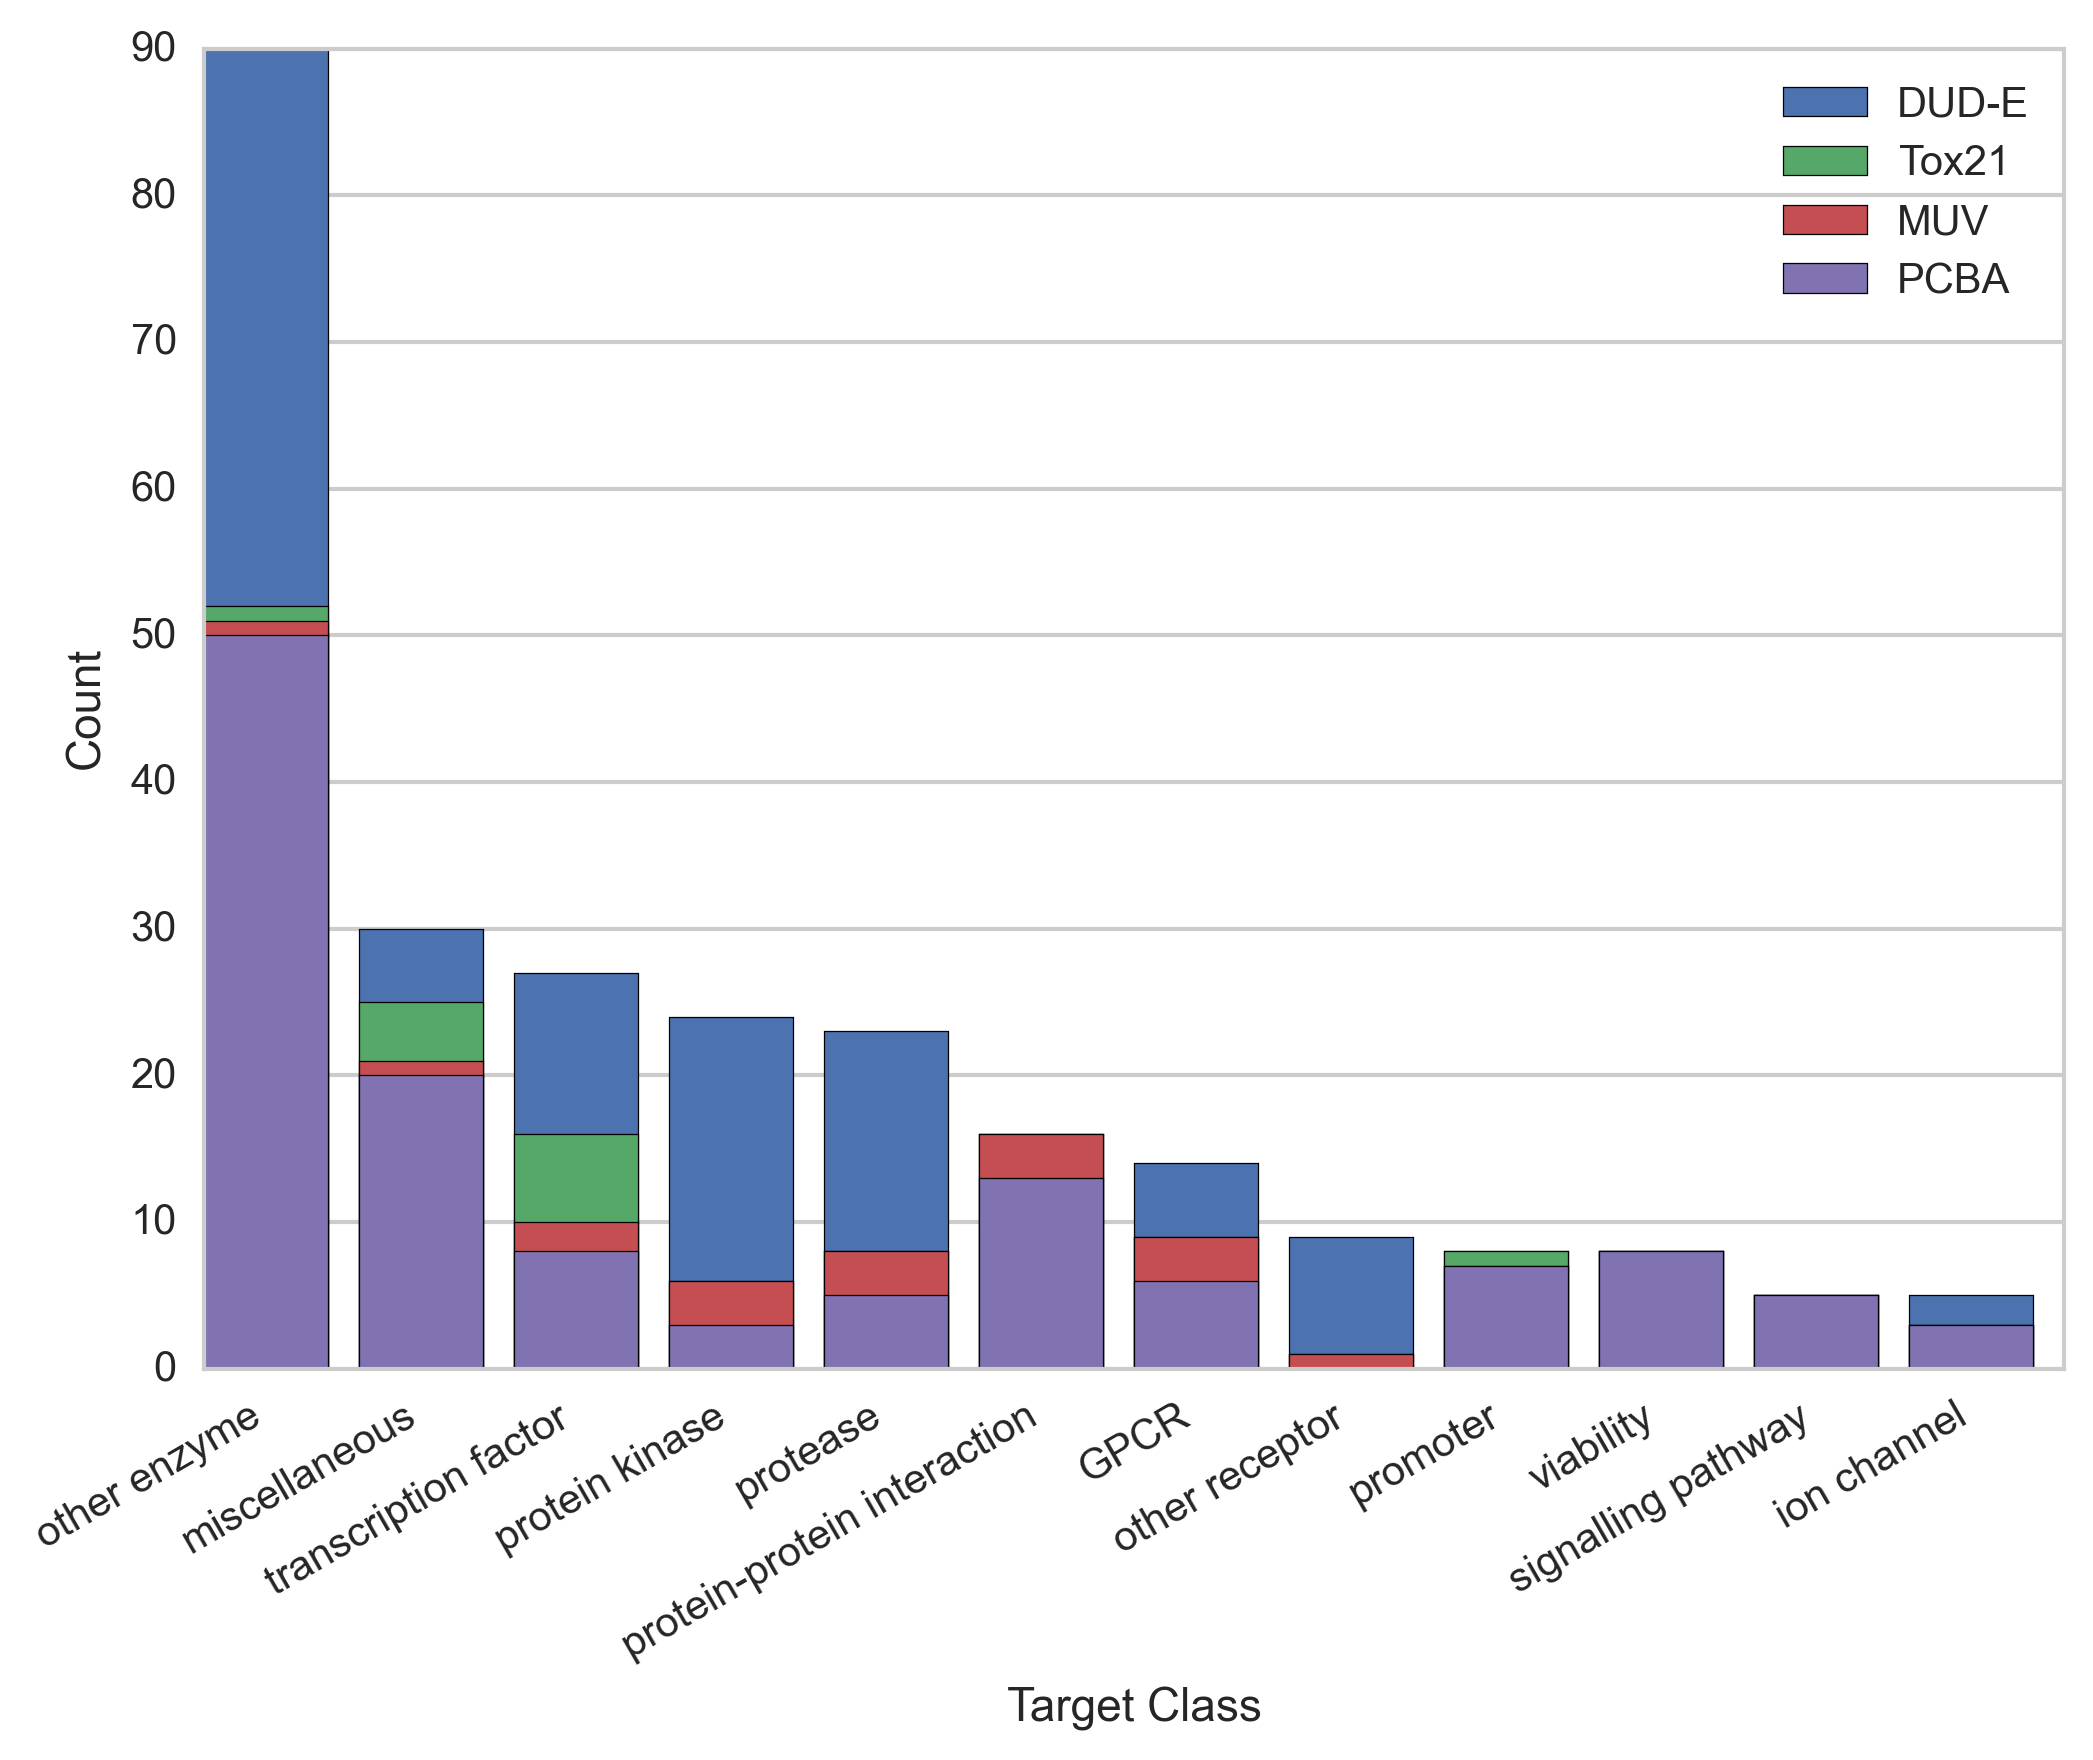
\includegraphics[width=\linewidth]{Images/target_bar.png}
\caption{Target class breakdown. Classes with fewer than five members were
  merged into the ``miscellaneous'' class.}
\label{fig:target_bar}
\end{figure}

\clearpage
\afterpage{%
\clearpage% Flush earlier floats (otherwise order might not be correct)
\thispagestyle{empty}% empty page style (?)
\begin{landscape}% Landscape page
\centering % Center table
\begin{table}[ht]
\centering
\caption{Held-in datasets.}
\label{tab:held-in}
\vskip 0.2in
\begin{tabular}{lSSll}
\toprule
\bfseries Dataset & \bfseries Actives & \bfseries Inactives & \bfseries Target Class & \bfseries Target \\
\midrule
pcba-aid899 & 1809 & 7575 & other enzyme & CYP2C19 \\
pcba-aid485297 & 9126 & 311481 & promoter & Rab9 \\
pcba-aid651644 & 748 & 361115 & miscellaneous & Vpr \\
pcba-aid651768 & 1677 & 362320 & other enzyme & WRN \\
pcba-aid743266 & 306 & 405368 & GPCR & PTHR1 \\
muv-aid466 & 30 & 14999 & GPCR & S1P1 receptor \\
muv-aid852 & 30 & 15000 & protease & FXIIa \\
muv-aid859 & 30 & 15000 & GPCR & M1 receptor \\
tox-NR-Aromatase & 300 & 5521 & other enzyme & Aromatase \\
tox-SR-MMP & 919 & 4891 & miscellaneous & mitochondrial membrane potential \\
\bottomrule
\end{tabular}
\end{table}

\begin{table}[ht]
\centering
\caption{Held-out datasets.}
\label{tab:held-out}
\vskip 0.2in
\begin{tabular}{lSSll}
\toprule
\bfseries Dataset & \bfseries Actives & \bfseries Inactives & \bfseries Target Class & \bfseries Target \\
\midrule
pcba-aid1461 & 2305 & 218561 & GPCR & NPSR \\
pcba-aid2675 & 99 & 279333 & miscellaneous & MBNL1-CUG \\
pcba-aid602233 & 165 & 380904 & other enzyme & PGK \\
pcba-aid624417 & 6388 & 398731 & GPCR & GLP-1 \\
pcba-aid652106 & 496 & 368281 & miscellaneous & alpha-synuclein \\
muv-aid548 & 30 & 15000 & protein kinase & PKA \\
muv-aid832 & 30 & 15000 & protease & Cathepsin G \\
muv-aid846 & 30 & 15000 & protease & FXIa \\
tox-NR-AhR & 768 & 5780 & transcription factor & Aryl hydrocarbon receptor \\
tox-SR-ATAD5 & 264 & 6807 & promoter & ATAD5 \\
\bottomrule
\end{tabular}
\end{table}
\end{landscape}
\clearpage% Flush page
}

\begin{figure}[ht]
\centering
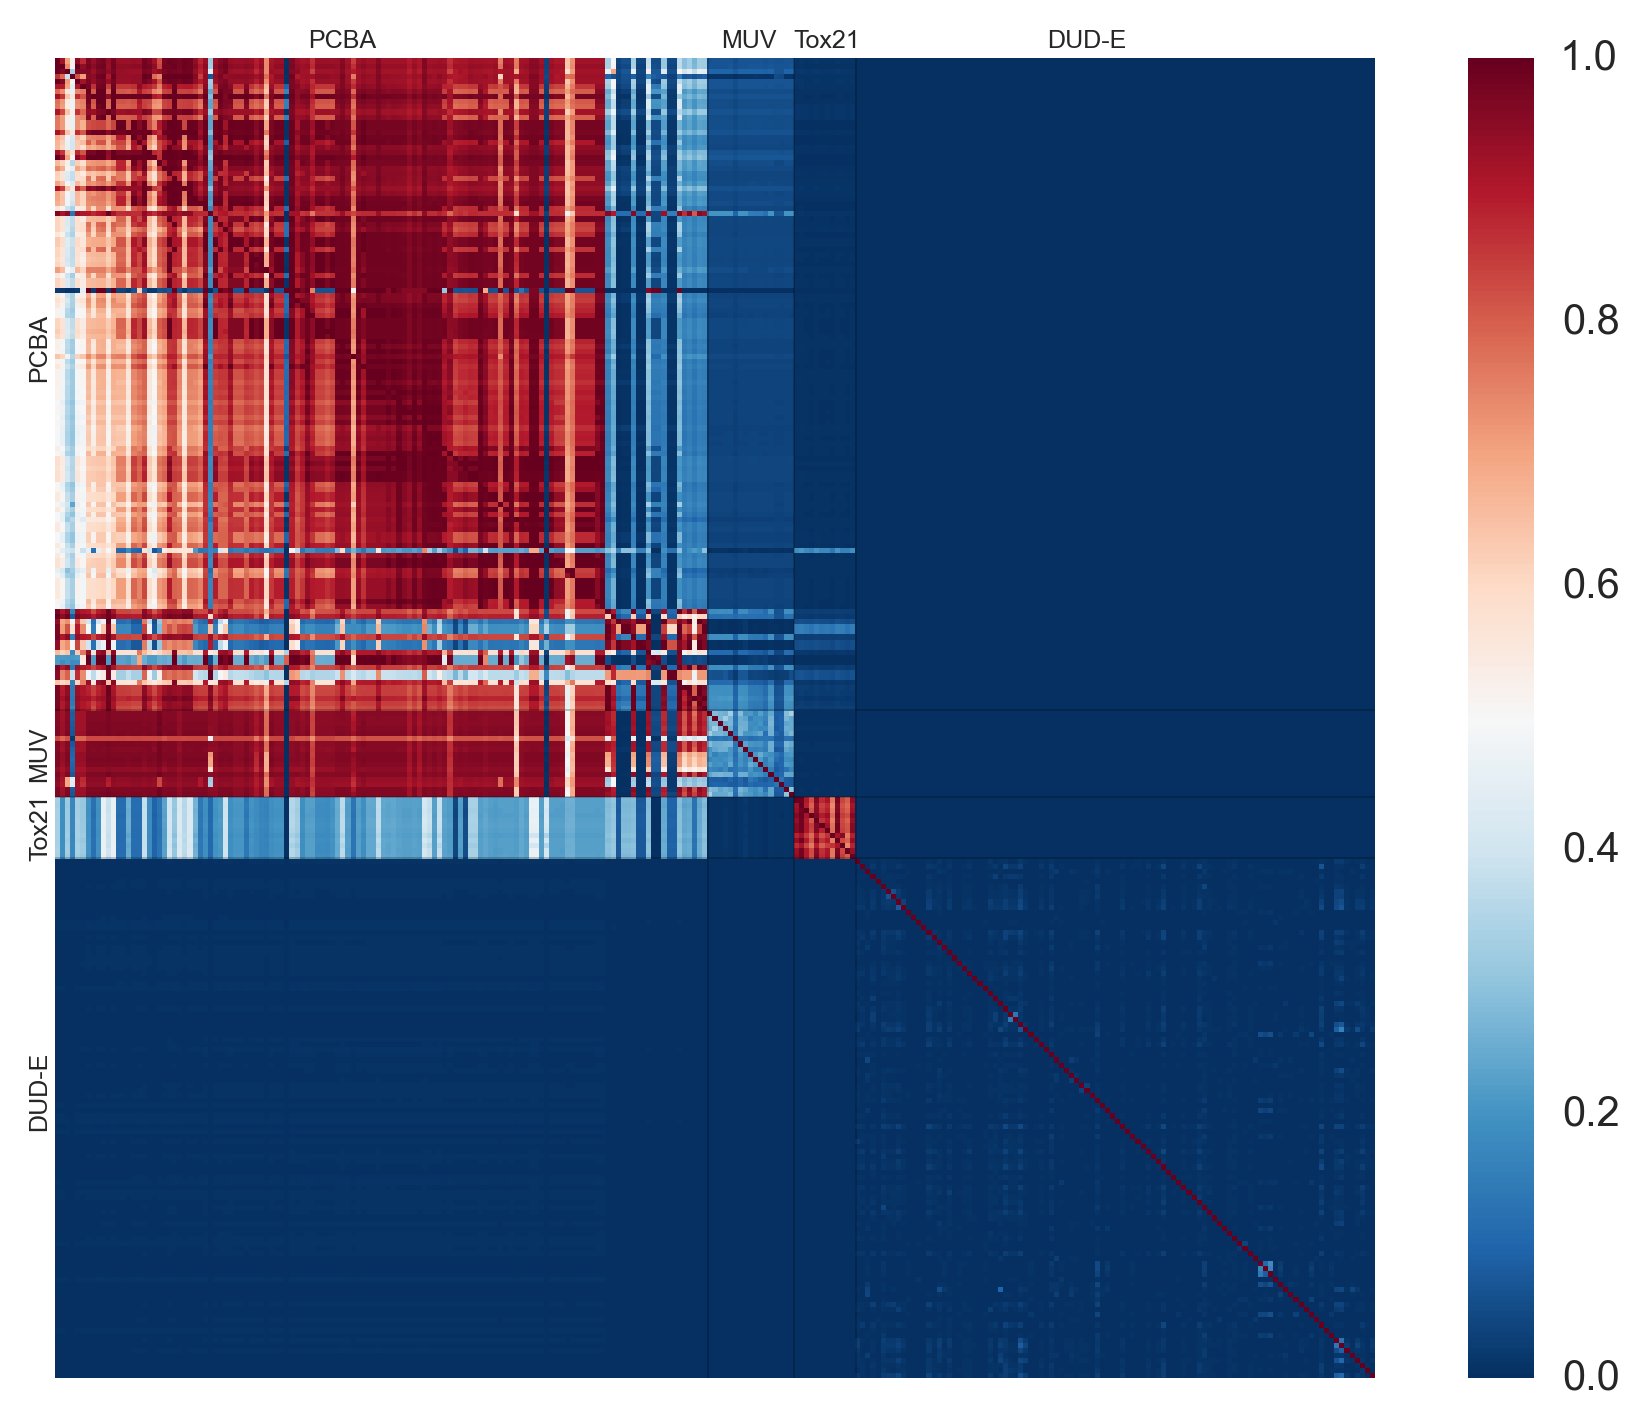
\includegraphics[width=\linewidth]{Images/dataset_heatmap.png}
\caption{Pairwise dataset intersections. The value of the element at
  position $(x, y)$ corresponds to the fraction of dataset $x$ that is
  contained in dataset $y$. Thin black lines are used to indicate divisions
  between dataset groups.}
\label{fig:dataset_heatmap}
\end{figure}

\begin{figure}[ht]
\centering
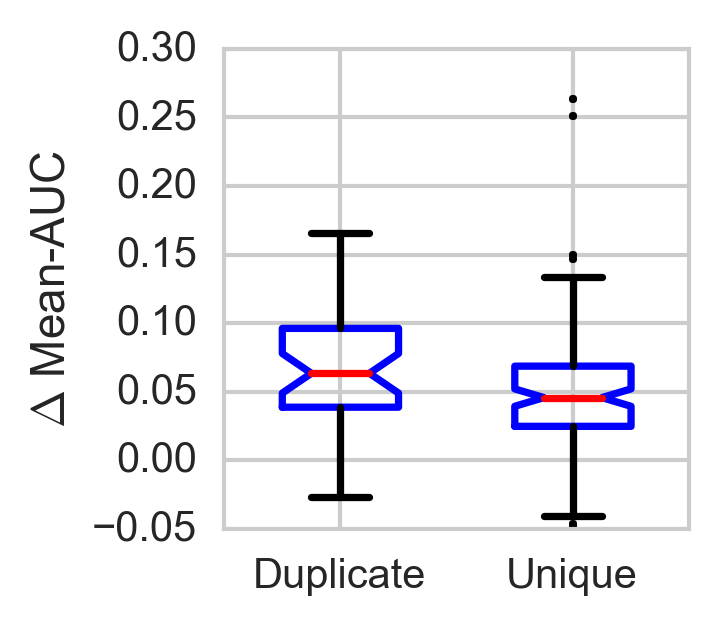
\includegraphics[width=0.5\linewidth]{Images/duplicate.png}
\caption{Multitask performance of duplicate and unique targets. Outliers
  are omitted for clarity. Notches indicate a confidence interval around the
  median, computed as $\pm 1.57 \times \text{IQR}/ \sqrt{N}$
  \citep{mcgill1978variations}.}
\label{fig:duplicates}
\end{figure}

\clearpage

\subsection{Performance metrics}

\begin{figure}[ht]
\centering
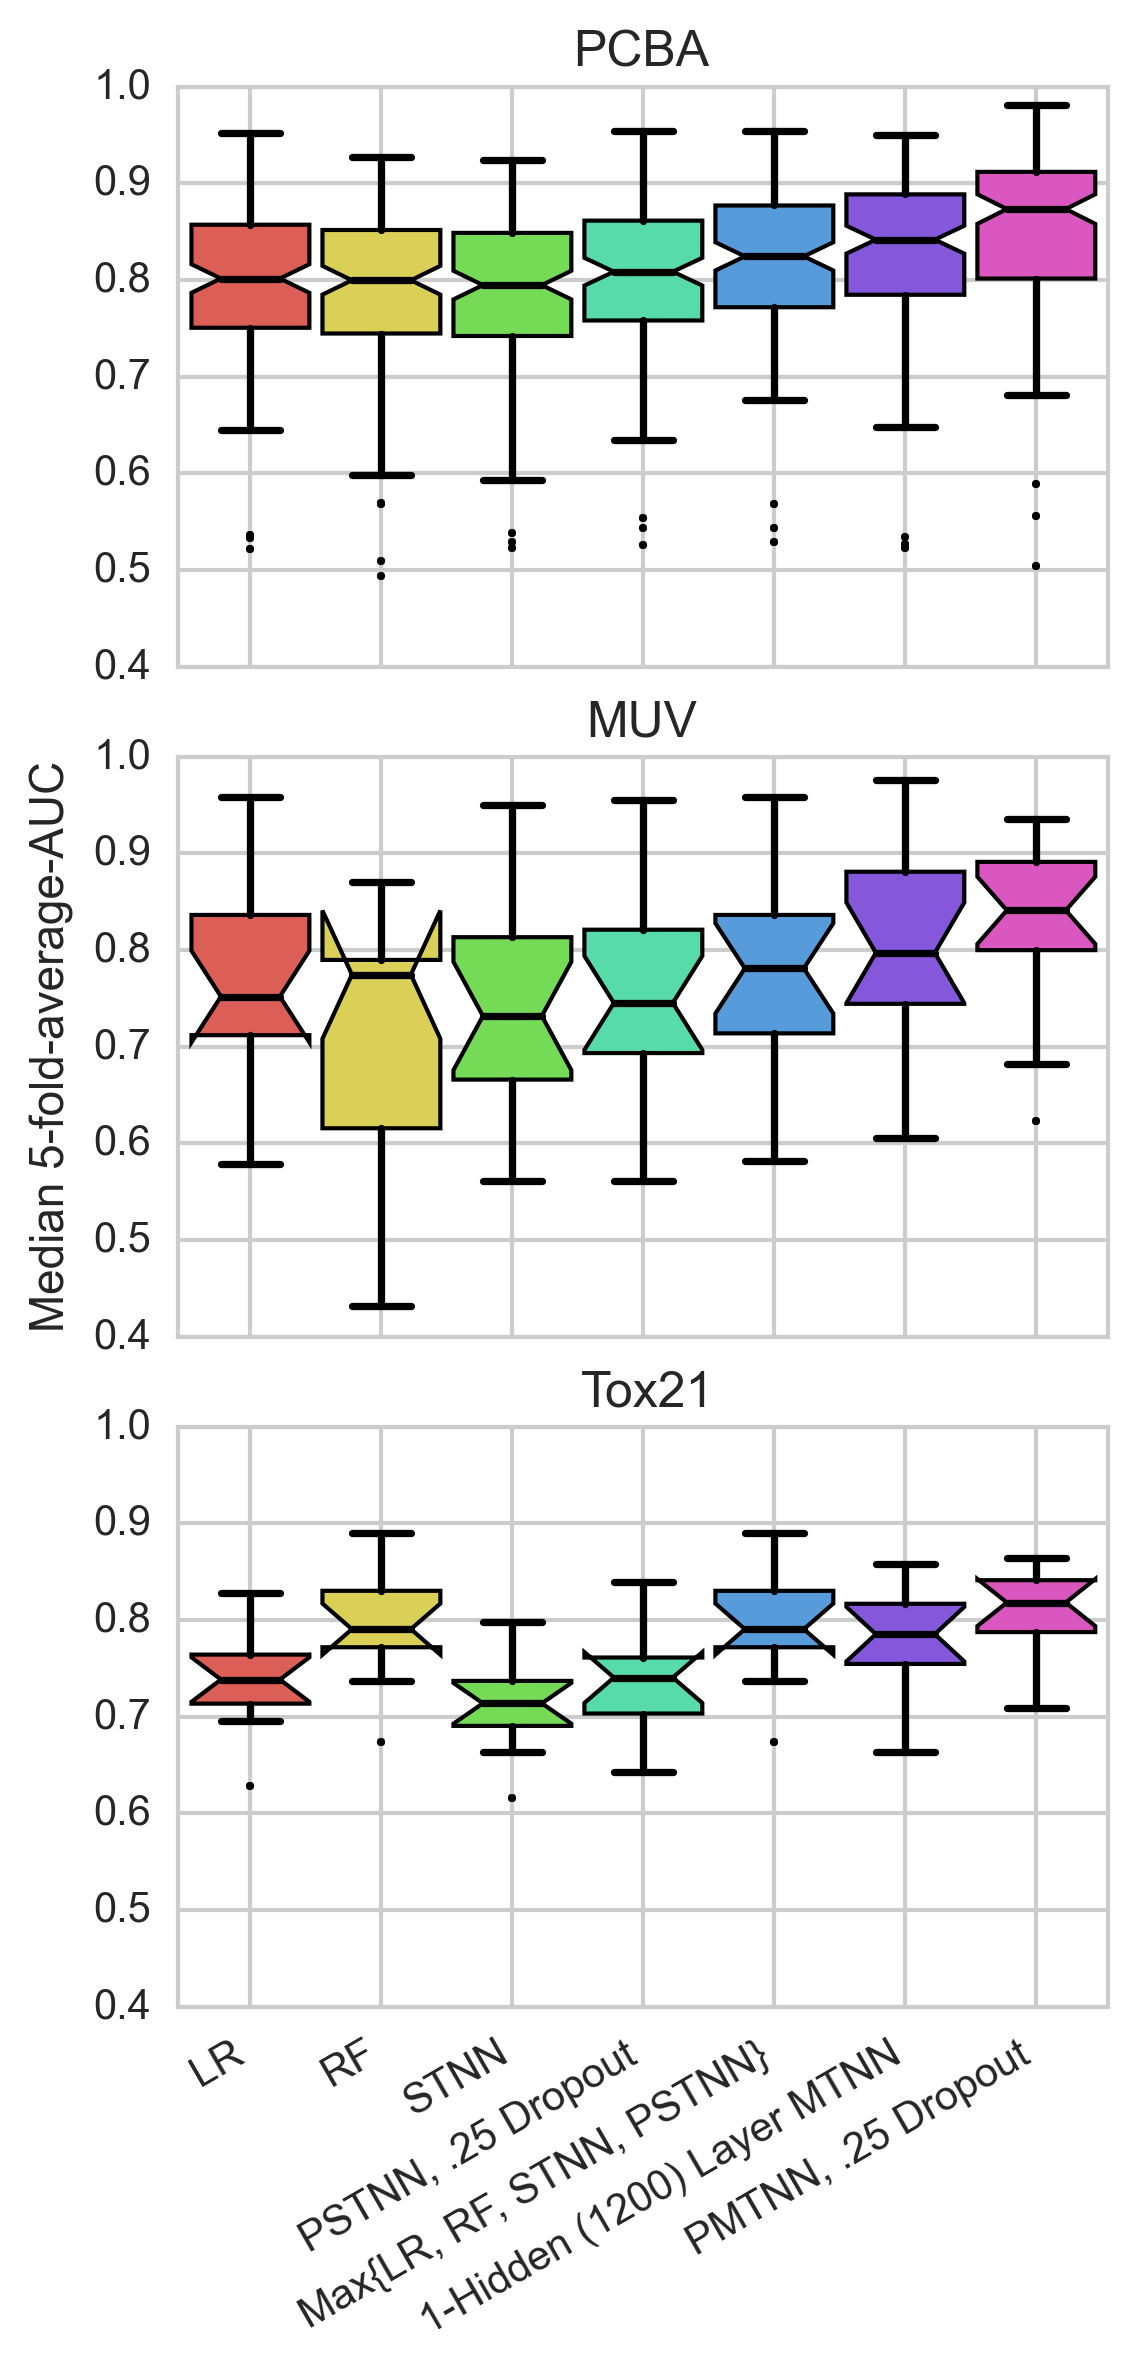
\includegraphics[height=0.9\textheight]{Images/table2boxplot.png}
\caption{Graphical representation of data from Table 2 in the text. Notches
  indicate a confidence interval around the median, computed as $\pm 1.57
  \times \text{IQR}/ \sqrt{N}$ \citep{mcgill1978variations}. Occasionally the
  notch limits go beyond the quartile markers, producing a ``folded down''
  effect on the boxplot. Paired $t$-tests (2-sided) relative to the PMTNN
  across all non-DUD-E datasets gave $p \le \num{1.86e-15}$.}
\label{fig:table2boxplot}
\end{figure}


\begin{table}[ht]
\centering
\caption{Sign test CIs for each group of datasets. Each model is compared
to the Pyramidal $(2000, 100)$ Multitask Neural Net, .25 Dropout model.}
\label{tab:sign-tests}
\vskip 0.2in
\begin{tabular}{ccccc}
\toprule
Model & \makecell{PCBA \\ $(n=128)$} & \makecell{MUV \\ $(n=17)$} & \makecell{Tox21 \\ $(n=12)$} \\
\midrule
Logistic Regression (LR)
& $[.3, .11]$ & $[.13, .53]$ & $[.00, .24]$ \\
Random Forest (RF)
& $[.05, .16]$ & $[.00, .18]$ & $[.14, .61]$ \\
Single-Task Neural Net (STNN)
& $[.02, .10]$ & $[.13, .53]$ & $[.00, .24]$ \\
Pyramidal $(2000, 100)$ STNN, .25 Dropout (PSTNN)
& $[.05, .15]$ & $[.13, .53]$ & $[.00, .24]$ & \\
Max\{LR, RF, STNN, PSTNN\}
& $[.09, .21]$ & $[.13, .53]$ & $[.14, .61]$ & \\
$1$-Hidden $(1200)$ Layer Multitask Neural Net (MTNN)
& $[.05, .15]$ & $[.22, .64]$ & $[.01, .35]$ & \\
%$4$-Hidden $(1000)$ Layer Multitask Neural Net
%& $[.05, .15]$ & $[.22, .64]$ & $[.25, .75]$ & \\
\bottomrule
\end{tabular}
\end{table}

\begin{table}[ht]
\centering
\caption{Enrichment scores for all models reported in Table~2. Each value
  is the median across the datasets in a group of the mean $k$-fold
  enrichment values. Enrichment is an alternate measure of model performance
  common in virtual drug screening. We use the ``ROC enrichment'' definition
  from~\cite{jain2008recommendations}, but roughly enrichment is the factor
  better than random that a model's top $X\%$ predictions are.}
\label{tab:enrichment}
\vskip 0.2in
\begin{tabular}{l|cccc|cccc|cccc}
\toprule
Model & \multicolumn{4}{|c|}{PCBA} & \multicolumn{4}{|c|}{MUV} &
 \multicolumn{4}{|c}{Tox21} \\
&
0.5\% & 1\% & 2\% & 5\% &
0.5\% & 1\% & 2\% & 5\% &
0.5\% & 1\% & 2\% & 5\% \\
\midrule
LR
& 19.4 &   16.5 &   12.1 &   7.9
& 20.0 &   23.3 &   15.0 &   8.0
& 23.9 &   18.3 &   10.6 &   6.7
\\
RF
& 40.0 &   27.4 &   17.4 &   9.1
& \textbf{40.0} &   \textbf{26.7} &   \textbf{16.7} &   7.3
& 23.2 &   \textbf{19.5} &   \textbf{13.6} &   7.8
\\
STNN
& 19.0 &   15.6 &   11.8 &   7.7
& 26.7 &   20.0 &   11.7 &   8.0
& 16.2 &   14.4 &   9.8  &   6.1
\\
PSTNN
& 21.8 &   16.9 &   12.4 &   7.9
& 26.7 &   16.7 &   13.3 &   8.0
& 23.8 &   16.1 &   10.0 &   6.7
\\
MTNN
& 33.8 &   23.6 &   16.9 &   9.8
& 26.7 &   16.7 &   \textbf{16.7} &   8.7
& \textbf{24.5} &   18.0 &   11.4 &   6.9
\\
PMTNN
& \textbf{43.8} &   \textbf{29.6} &   \textbf{19.7} &   \textbf{11.2}
& \textbf{40.0} &   23.3 &   \textbf{16.7} &   \textbf{10.0}
& 23.5 &   18.5 &   \textbf{13.7} &   \textbf{8.1}
\\
\bottomrule
\end{tabular}
\end{table}

\clearpage

\subsection{Training Details}
The multitask networks in Table 2 were trained with learning rate $.0003$
and batch size $128$ for $50$M steps using stochastic gradient descent.
Weights were initialized from a zero-mean Gaussian with standard deviation
$.01$. The bias was initialized at $.5$. We experimented with higher
learning rates, but found that the pyramidal networks sometimes failed to
train (the top hidden layer zeroed itself out). However, this effect
vanished with the lower learning rate.  Most of the models were trained
with 64 simultaneous replicas sharing their gradient updates, but in some
cases we used as many as 256.

The pyramidal single-task networks were trained with the same settings, but
for $100$K steps. The vanilla single-task networks were trained with
learning rate $.001$ for $100$K steps. The networks used in Figure 3 and
Figure 4 were trained with learning rate $0.003$ for 500 epochs plus a
constant 3 million steps. The constant factor was introduced after we
observed that the smaller multitask networks required more epochs than the
larger networks to stabilize.

The networks in Figure~5 were trained with a Pyramidal (1000, 50) Single
Task architecture (matching the networks in Figure~3). The weights were
initialized with the weights from the networks represented in Figure~3 and
then trained for 100K steps with a learning rate of 0.0003.

As we noted in the main text, the datasets in our collection contained many
more inactive than active compounds. To ensure the actives were given
adequate importance during training, we weighted the actives for each
dataset so that they had total weight equal to the number of inactives for
that dataset (inactives were given unit weight).

\tablename~\ref{tab:sensitivity} contains the results of our pyramidal
model sensitivity analysis.  Tables \ref{tab:model_descriptions} and
\ref{tab:models} give results for a variety of additional models not
reported in Table 2.

\begin{table}[ht]
\centering
\caption{Pyramid sensitivity analysis. Median 5-fold-average-AUC values are
  given for several variations of the pyramidal architecture. In an attempt
  to avoid the problem of training failures due to the top layer becoming all
  zero early in the training, the learning rate was set to 0.0001 for the
  first 2M steps then to 0.0003 for 28M steps.}
\label{tab:sensitivity}
\vskip 0.2in
\begin{tabular}{l >{$}c<{$} >{$}c<{$} >{$}c<{$} }
\toprule
\textnormal{Model} & \makecell{\text{PCBA} \\ (n=128)} & \makecell{\text{MUV} \\ (n=17)} & \makecell{\text{Tox21} \\ (n=12)} \\
\midrule
Pyramidal $(1000, 50)$ MTNN & .846 & .825 & .799 \\
Pyramidal $(1000, 100)$ MTNN & .845 & .818 & .796 \\
Pyramidal $(1000, 150)$ MTNN & .842 & .812 & .798 \\
Pyramidal $(2000, 50)$ MTNN & .846 & .819 & .794 \\
Pyramidal $(2000, 100)$ MTNN & .846 & .821 & .798 \\
Pyramidal $(2000, 150)$ MTNN & .845 & .839 & .792 \\
Pyramidal $(3000, 50)$ MTNN & .848 & .801 & .796 \\
Pyramidal $(3000, 100)$ MTNN & .844 & .804 & .799 \\
Pyramidal $(3000, 150)$ MTNN & .843 & .810 & .789 \\
\bottomrule
\end{tabular}
\end{table}

\clearpage

\begin{table}[ht]
\centering
\caption{Descriptions for additional models. MTNN: multitask neural net.
  ``Auxiliary heads'' refers to the attachment of independent softmax units
  for each task to hidden layers \cite[see][]{szegedy2014going}. Unless
  otherwise marked, assume 10M training steps.}
\label{tab:model_descriptions}
\vskip 0.2in
%\begin{tabular}{>{\bfseries}cp{6in}}
\begin{tabular}{>{\bfseries}cl}
\toprule
A & $8$-Hidden $(300)$ Layer MTNN, auxiliary heads attached to hidden layers 3 and 6, 6M steps \\
B & $1$-Hidden $(3000)$ Layer MTNN, 1M steps \\
C & $1$-Hidden $(3000)$ Layer MTNN, 1.5M steps \\
D & Pyramidal $(1800, 100)$, 2 deep, reconnected (original input concatenated to first pyramid output) \\
E & Pyramidal $(1800, 100)$, 3 deep \\
F & $4$-Hidden $(1000)$ Layer MTNN, auxiliary heads attached to hidden layer 2, 4.5M steps \\
G & Pyramidal $(2000, 100)$ MTNN, 10\% connected \\
H & Pyramidal $(2000, 100)$ MTNN, 50\% connected \\
I & Pyramidal $(2000, 100)$ MTNN, $.001$ learning rate \\
J & Pyramidal $(2000, 100)$ MTNN, 50M steps, $.0003$ learning rate \\
K & Pyramidal $(2000, 100)$ MTNN, $.25$ Dropout (first layer only), 50M steps \\
L & Pyramidal $(2000, 100)$ MTNN, $.25$ Dropout, $.001$ learning rate \\
\bottomrule
\end{tabular}
\end{table}

\begin{table}[ht]
\centering
\caption{Median 5-fold-average AUC values for additional models. Sign test
  confidence intervals and paired $t$-test (2-sided) $p$-values are relative
  to the PMTNN from Table 2 and were calculated across all non-DUD-E
  datasets.}
\label{tab:models}
\vskip 0.2in
\begin{tabular}{ >{\bfseries}c >{$}c<{$} >{$}c<{$} >{$}c<{$} >{$}c<{$} >{$}c<{$} }
\toprule
\textnormal{Model} & \makecell{\text{PCBA} \\ (n=128)} & \makecell{\text{MUV} \\ (n=17)} & \makecell{\text{Tox21} \\ (n=12)} & \text{Sign Test CI} & \text{Paired $t$-Test} \\
\midrule
A & .836 & .793 & .786 & [.01, .06] & \num{9.37e-43} \\
B & .835 & .855 & .769 & [.11, .22]  & \num{1.17e-17} \\
C & .837 & .851 & .765 & [.12, .24] & \num{2.60e-16} \\
D & .842 & .842 & .816 & [.08, .18] & \num{1.89e-21} \\
E & .842 & .808 & .789 & [.02, .08] & \num{9.25e-43} \\
F & .858 & .836 & .810 & [.10, .22] & \num{4.85e-13} \\
G & .831 & .795 & .774 & [.03, .11] & \num{1.15e-31} \\
H & .856 & .827 & .796 & [.04, .13] & \num{5.34e-21} \\
I & .860 & .862 & .824 & [.07, .17] & \num{6.23e-14} \\
J & .830 & .810 & .801 & [.05, .14] & \num{9.25e-25} \\
K & .859 & .843 & .803 & [.24, .38] & \num{3.25e-9} \\
L & .872 & .837 & .802 & [.35, .50] & \num{2.74e-2} \\
\bottomrule
\end{tabular}
\end{table}

\clearpage

\subsection{Active Occurrence Rate (AOR)}

\figurename~\ref{fig:dataset_similarity} plots multitask improvement against a
measure of dataset similarity we call ``active occurrence rate''. For each
active compound $\alpha$ in dataset $D_i$, $\text{AOR}_{i,\alpha}$ is defined as
the number of additional datasets in which this compound is also active:
\[
\text{AOR}_{i, \alpha} = \sum_{d \neq i} \mathbbm{1}{\left(\alpha \in \text{Actives}\left(D_d\right)\right)}.
\]
Each point in \figurename~\ref{fig:dataset_similarity} corresponds to a
single dataset $D_i$. The $x$-coordinate is
\[
\text{AOR}_i = \Mean_{\alpha \in \text{Actives}\left(D_i\right)}\left(\text{AOR}_{i, \alpha}\right),
\]
and the $y$-coordinate is ($\Delta$ mean-AUC) between multitask and
single-task models. Note that DUD-E was excluded from this analysis.

\begin{figure}[ht]
\centering
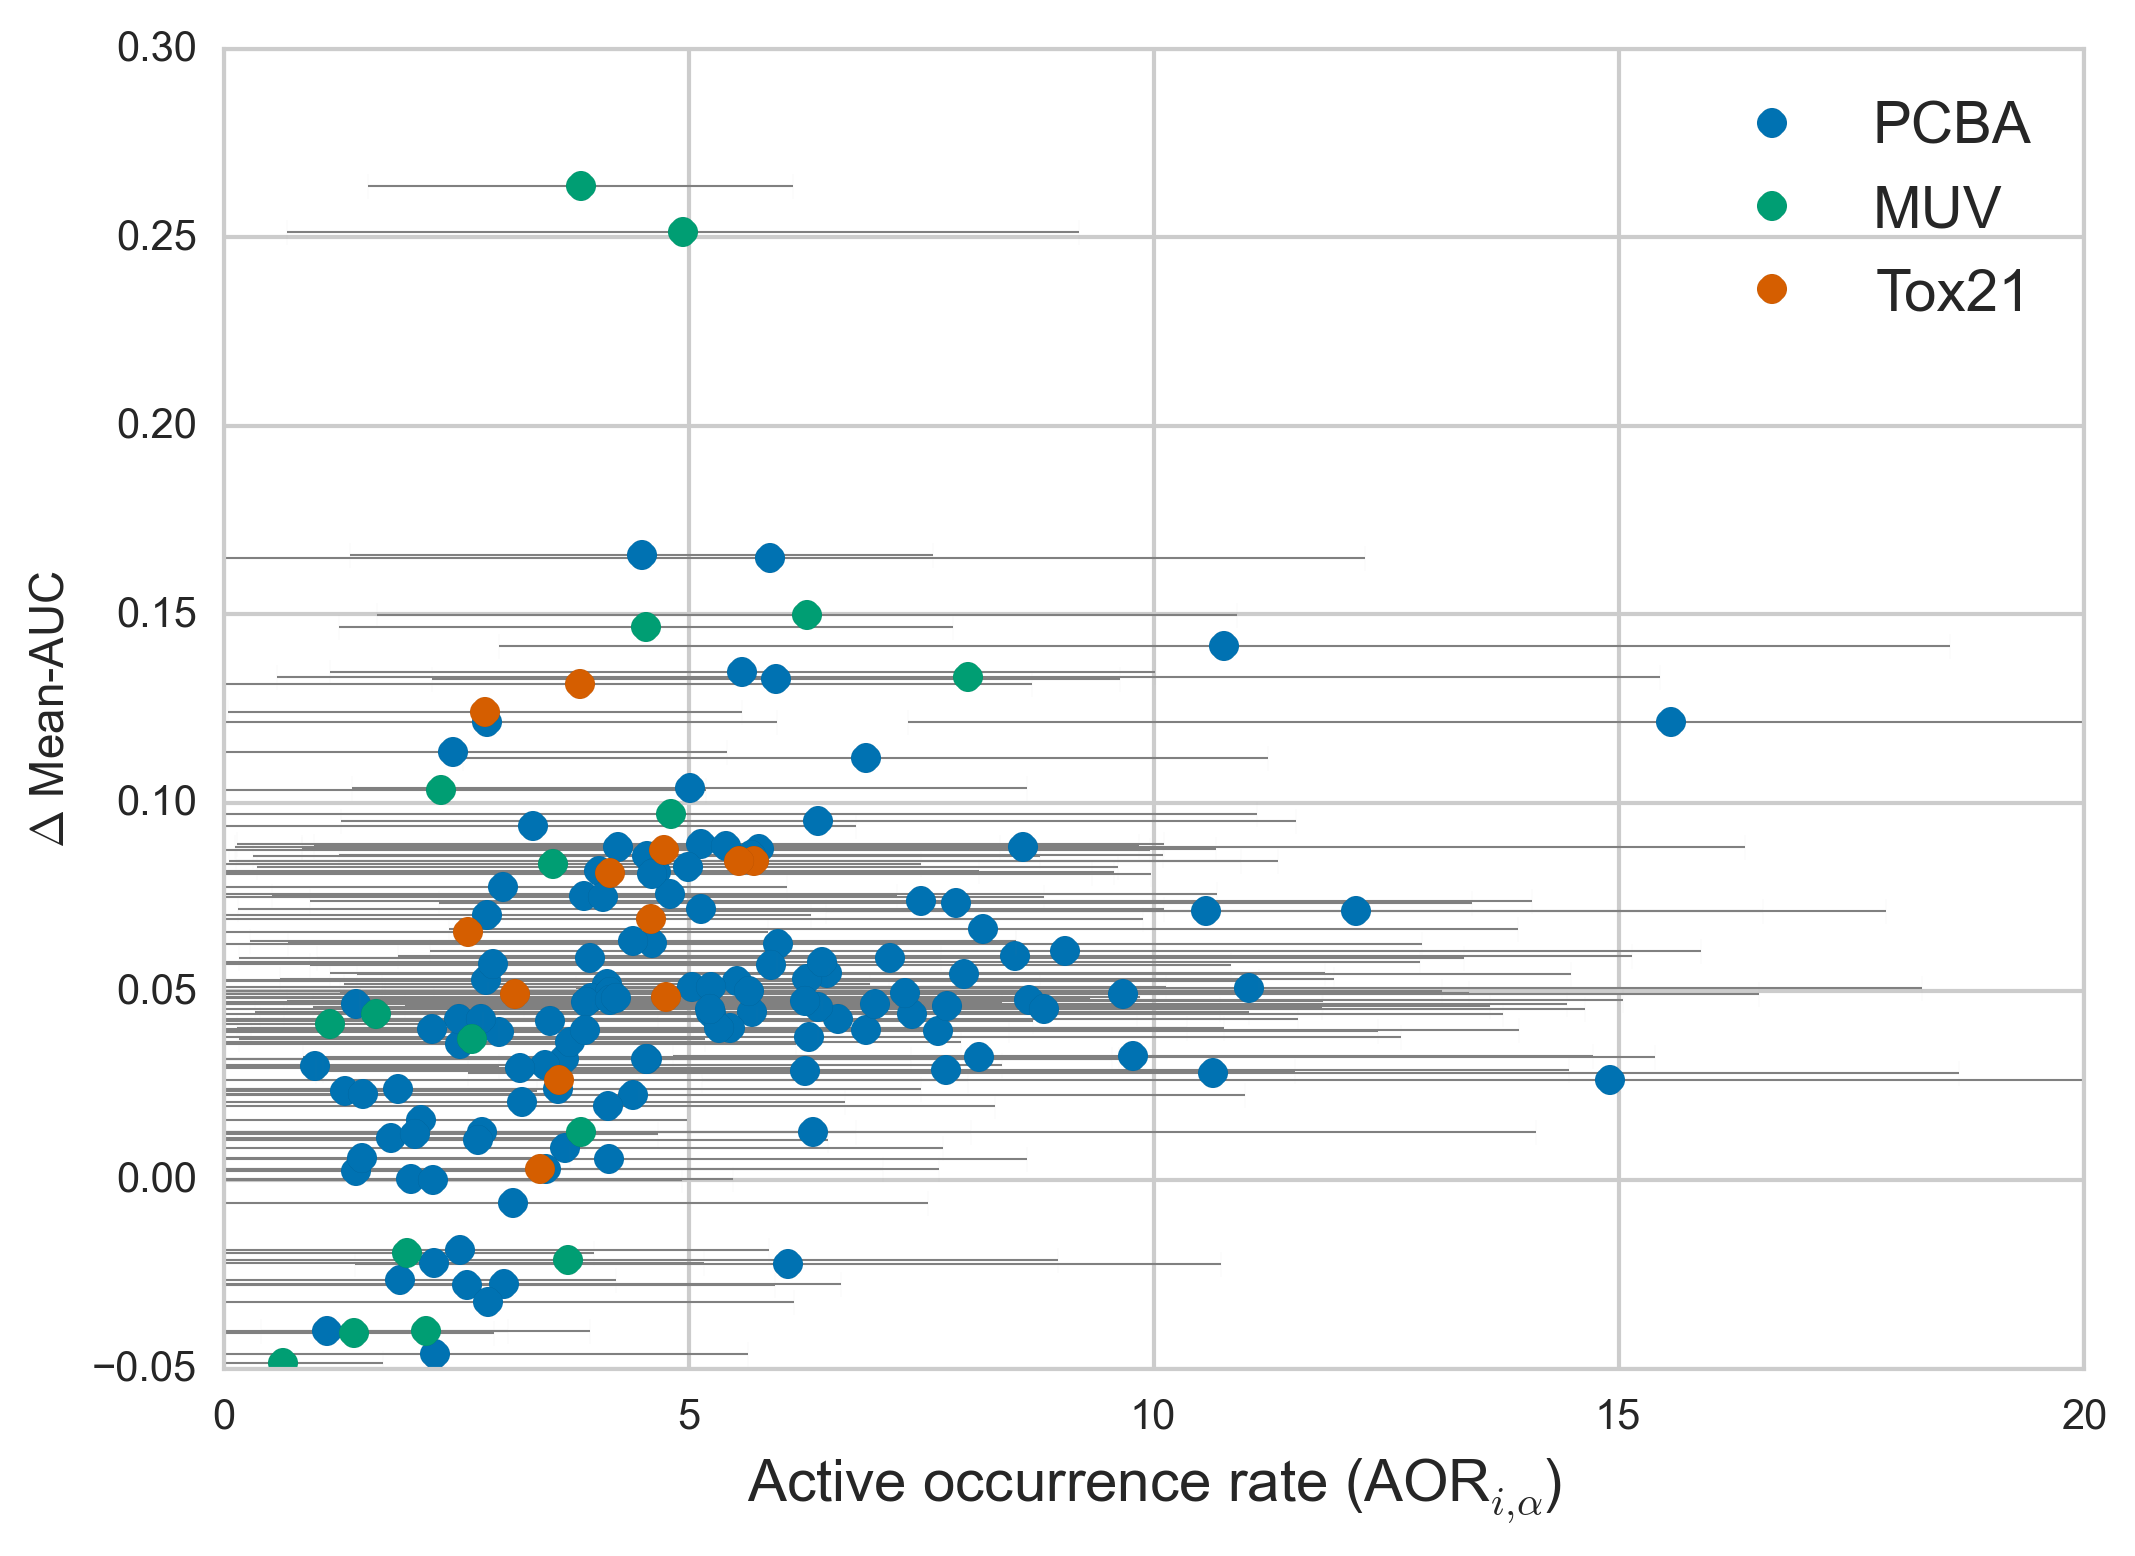
\includegraphics[width=0.9\linewidth]{Images/dataset_similarity.png}
\caption{Multitask improvement compared to active occurrence rate (AOR).
  Each point in the figure represents a particular dataset $D_i$. The
  $x$-coordinate is the mean AOR across all active compounds in $D_i$, and
  the $y$-coordinate is the difference in mean-AUC between
  multitask and single-task models. The gray bars indicate standard
  deviations around the AOR means. Note that DUD-E was excluded from this
  analysis.}
\label{fig:dataset_similarity}
\end{figure}

%\bibliography{appendix}
%\bibliographystyle{icml2015}

%\end{document}